\section{Auswertung}

Um die Extinktionsspektren zu erzeugen wurde das Ethanol/Ethanol Transmissionspektrum $\text{I}_{\text{Leer}}$ (siehe Abbildung \ref{fig:I_Leer}) jeweils durch die Transmissionsspektren $\text{I}_{\text{Substanz}}$ (siehe Abbildung \ref{fig:I_alleTrans}), welche verschiedenen Konzentrationen des Kristallvioletts gelöst in Ethanol enthielten, dividiert und anschließend der dekadische Logarithmus aus dem Quotienten gebildet. Die erhaltenen Extinktionsgraphen wurden in Abbildung~\ref{fig:Extinktionalle} aufgetragen. Es wurde angenommen, dass in der Analyse die Messungenauigkeit der Waage die größte Fehlerquelle darstellt. Deshalb wurde die Fehlerbetrachtung lediglich am Ende des Abschnitts gesamt durchgeführt. Die Absorbtion der $8 \cdot 10^{-5} \frac{mol}{L}$ Probe war so stark, dass keine diskreten Werte im Bereich des Maximums gefunden werden konnten. In der Abbildung wurde daher bei einer Extinktion von 3 der Graph abgeschnitten, um die restlichen Maxima besser erkennen zu können.
\begin{figure}[H]
	\centering	
	\begin{minipage}{1\textwidth}
	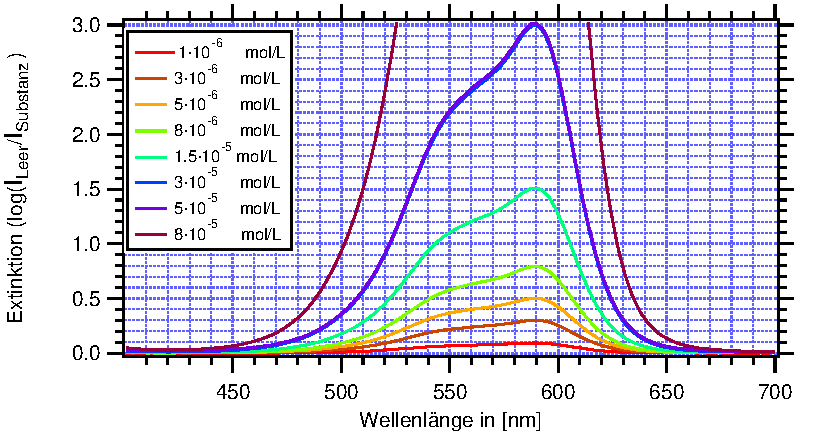
\includegraphics[width=\columnwidth]{Rohdaten/alleExtinktionenzusammen.pdf}	
	\caption{Extinktionen einer Kristallviolett/Ethanol Lösung verschiedener Konzentrationen. Die zugrundeliegenden Transmissionsmessungen wurden mit einem JASCO V-750 Spektrometer aufgenommen unter Verwendung von PMMA Küvetten mit einer Wegstrecke $L=10 \si{mm}$. Die Graphik wurde mit Igor Pro 6.37 erstellt.}
	\label{fig:Extinktionalle}
	\end{minipage}
	
\end{figure}

Durch das Anlegen eines \textit{off set} konnte mithilfe des Programms \textit{Igor Pro 6.37} die Extension am Absorbtionsmaximum für jede Konzentration abgelesen werden. Das Absorptionsmaximum wurde bei $598 \si{nm}$ gefunden. Hierfür wurde der Abstand des Extrema zum \textit{off set} bestimmt. Die Werte wurden in Tabelle \ref{tab:ExtMax} zusammengefasst.
\begin{table}[H]
	\centering
	\caption{Ermittelte Extension am Absorptionsmaximum aller unterschiedlichen, gemessenen Konzentrationen. Die Werte wurden als Differenz der Kurve zum Wert erhalten}
	\begin{tabular}{|C{0.25\linewidth}|C{0.25\linewidth}|}
		\hline \addlinespace[1ex] 
		Konzentration $\left[\si{\frac{mol}{L}}\right] $ &  Extension \\
		\hline \addlinespace[1ex] 
		$1\cdot 10^{-6}$ & 0.0910 \\
		$3\cdot 10^{-6}$ &0.2978\\
		$5\cdot 10^{-6}$ &0.4993\\
		$8\cdot 10^{-6}$ &0.7912\\
		$15\cdot 10^{-6}$ &1.5088\\
		$30\cdot 10^{-6}$ &2.9955\\
		$50\cdot 10^{-6}$ &3.1669\\
		$80\cdot 10^{-6}$ &5.0021\\
		\hline \addlinespace[1ex]  
	\end{tabular}
\label{tab:ExtMax}
\end{table}
Die so erhaltenen Wertepaare wurden anschließend mit dem Programm \textit{python 3} gegeneinander aufgetragen um eine diskrete Funktion der Extension über der Konzentration zu erhalten. Anschließend wurde durch die ersten sechs, als linear anzunehmende Wertepaare eine lineare Regression durchgeführt. Dieses Vorgehen wird in Abbildung \ref{fig:KonzgegenExt} gezeigt. \\
\begin{figure}[H]
	\centering	
	\begin{minipage}{1\textwidth}
		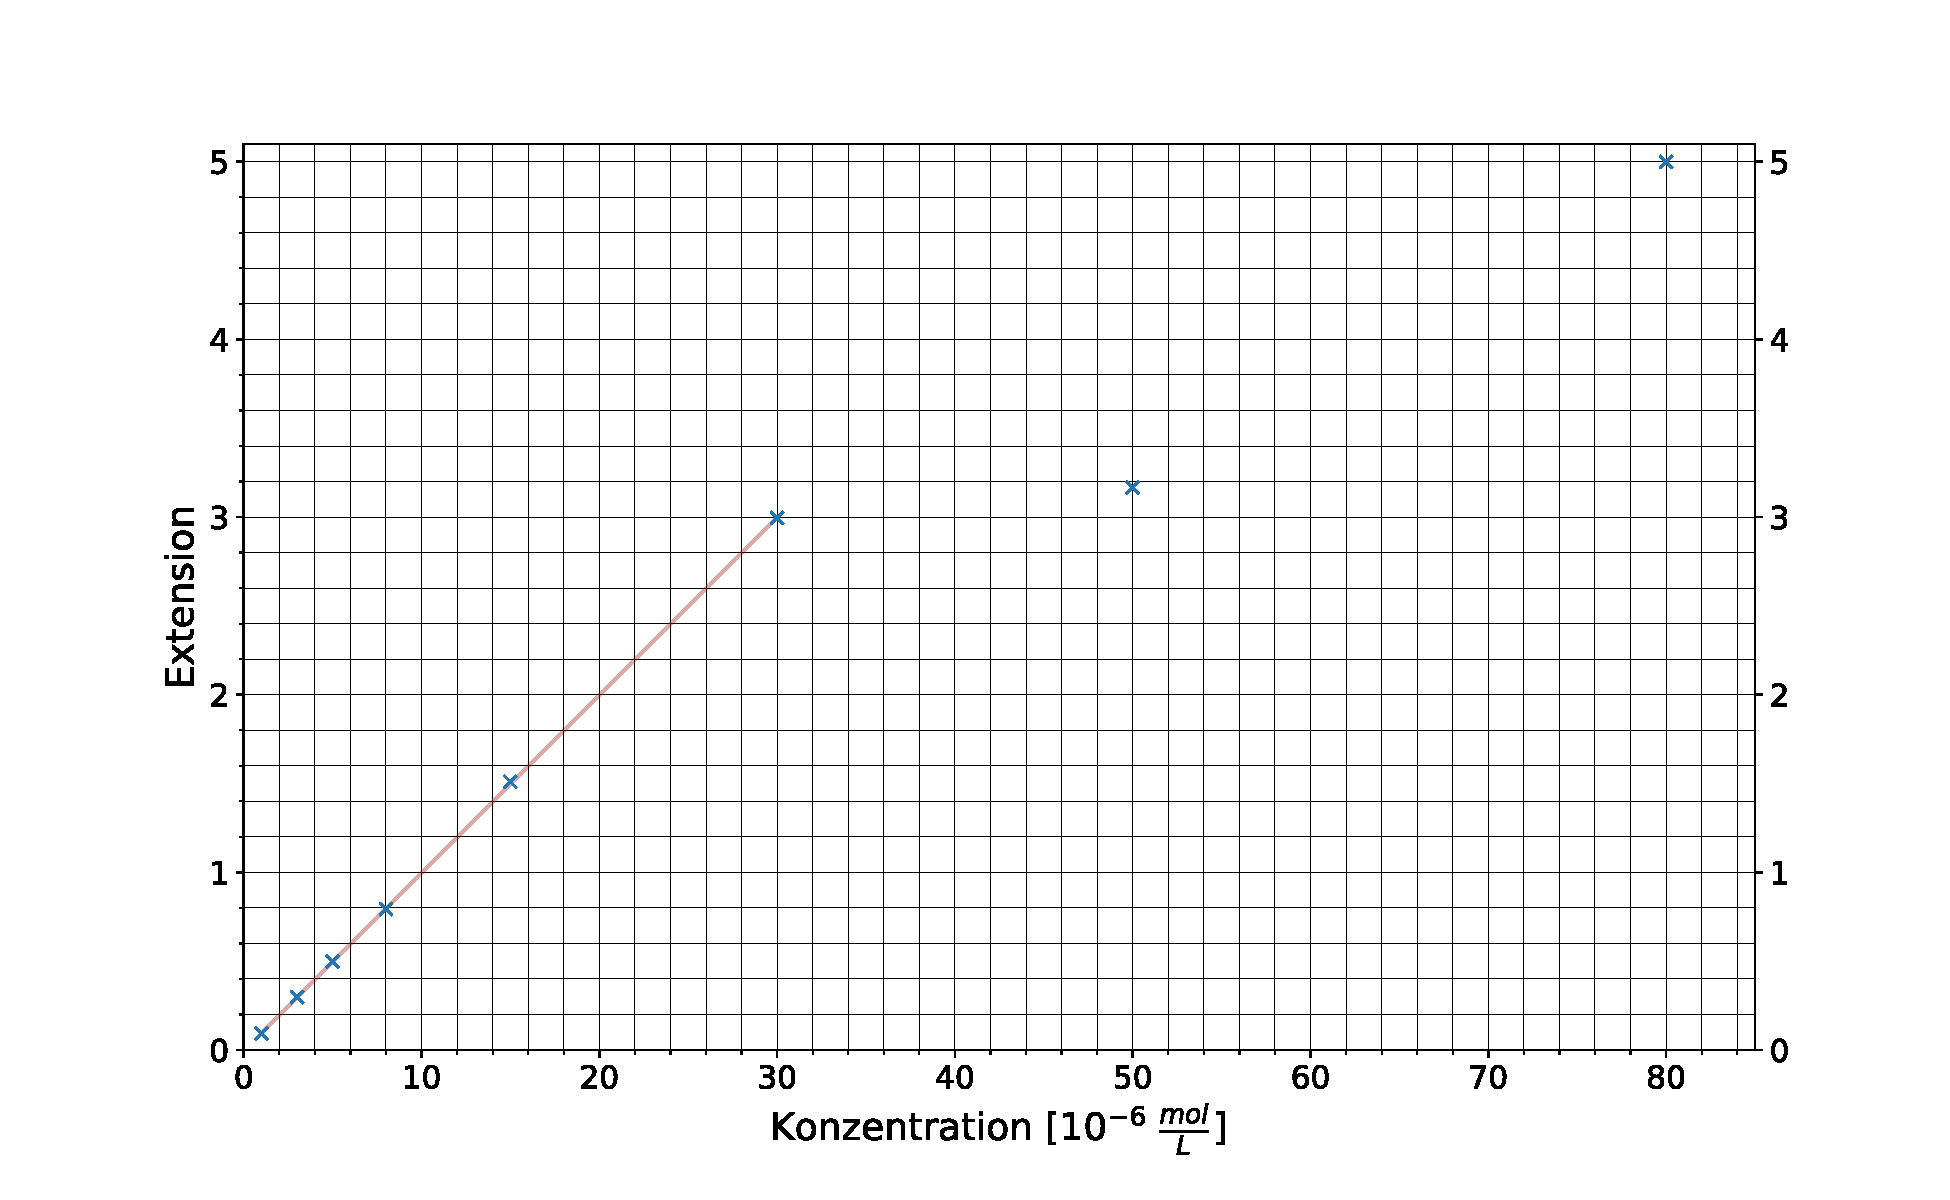
\includegraphics[width=\columnwidth]{Rohdaten/KonzgegenExt.pdf}	
		\caption{Auftragung der Extension am Maximum (bei 598$\,\si{nm}$) gegen die Konzentration. In rot ist die Ausgleichsgerade der durchgeführten linearen Regression der sechs ersten Werte dargestellt. Abbildung und Regression wurden in \textit{python 3} durchgeführt.}
		\label{fig:KonzgegenExt}
	\end{minipage}
	
\end{figure}
Die Steigung der vorliegenden Ausgleichsgerade entspricht nach Gleichung \ref{LambertBeer} in einer Näherung dem Produkt aus dekadische Extinktionskoeffizient sowie Küvettenlänge. Die Näherung resultiert aus der hohen Verdünnung der betrachteten Lösungen, also dem linear anzunehmenden Verlauf der Extinktion mit der Konzentration. Das exemplarisch gezeigte Vorgehen wurde für 13 weitere Wellenlängen im Abstand von ungefähr $10 \si{nm}$ wiederholt um molare dekadische Extinktionskoeffizienten für unterschiedliche Wellenlängen zu erhalten. Die Graphen zu den weiteren Wellenlängen zeigen gleiche Trends und werden hier nicht explizit gezeigt. Für eine gegebene Küvettenlänge von $10\si{mm}$ ergeben sich für die 14 betrachteten Wellenlängen in Tabelle \ref{} gezeigte dekadische Extinktionskoeffizient. Da die Einheit $\left[ \si{\frac{L}{mol\cdot cm}}\right]$ für die dekadische Extinktionskoeffizient eine gängige Darstellung ist, werden die Ergebnisse in dieser Einheit gezeigt.

\begin{table}[H]
	\centering
	\caption{Ermittelte dekadischen Extinktionskoeffizient für verschiedene Wellenlängen}
	\begin{tabular}{|C{0.25\linewidth}|C{0.3\linewidth}|}
		\hline \addlinespace[1ex] 
		Wellenlänge $[\si{nm}] $ &  molare dekadische Extinktionskoeffizient $\left[ 10^{3} \cdot \si{\frac{L}{mol\cdot cm}}\right]$  \\
		\hline \addlinespace[1ex] 
		510.7 & 1.21 \\
		520.6 &1.93\\
		530.6 &3.06\\
		540.6  &4.63\\
		550.5 & 6.27 \\
		560.6 &7.37\\
		570.4 &8.57\\
		580.4  &9.40\\		
		590.4 & 9.99 \\
		598.0 &10.01\\
		600.3 &8.32\\
		610.3 &4.98\\
		620.2  &2.33\\
		630.2 & 0.96 \\
		\hline \addlinespace[1ex]  
	\end{tabular}
	\label{tab:ExtKoeff}
\end{table}
Werden die molaren dekadischen Extinktionskoeffizienten über der Wellenlänge aufgetragen ergibt sich Abbildung \ref{fig:ExtKoeffs}.
\begin{figure}[H]
	\centering	
	\begin{minipage}{1\textwidth}
		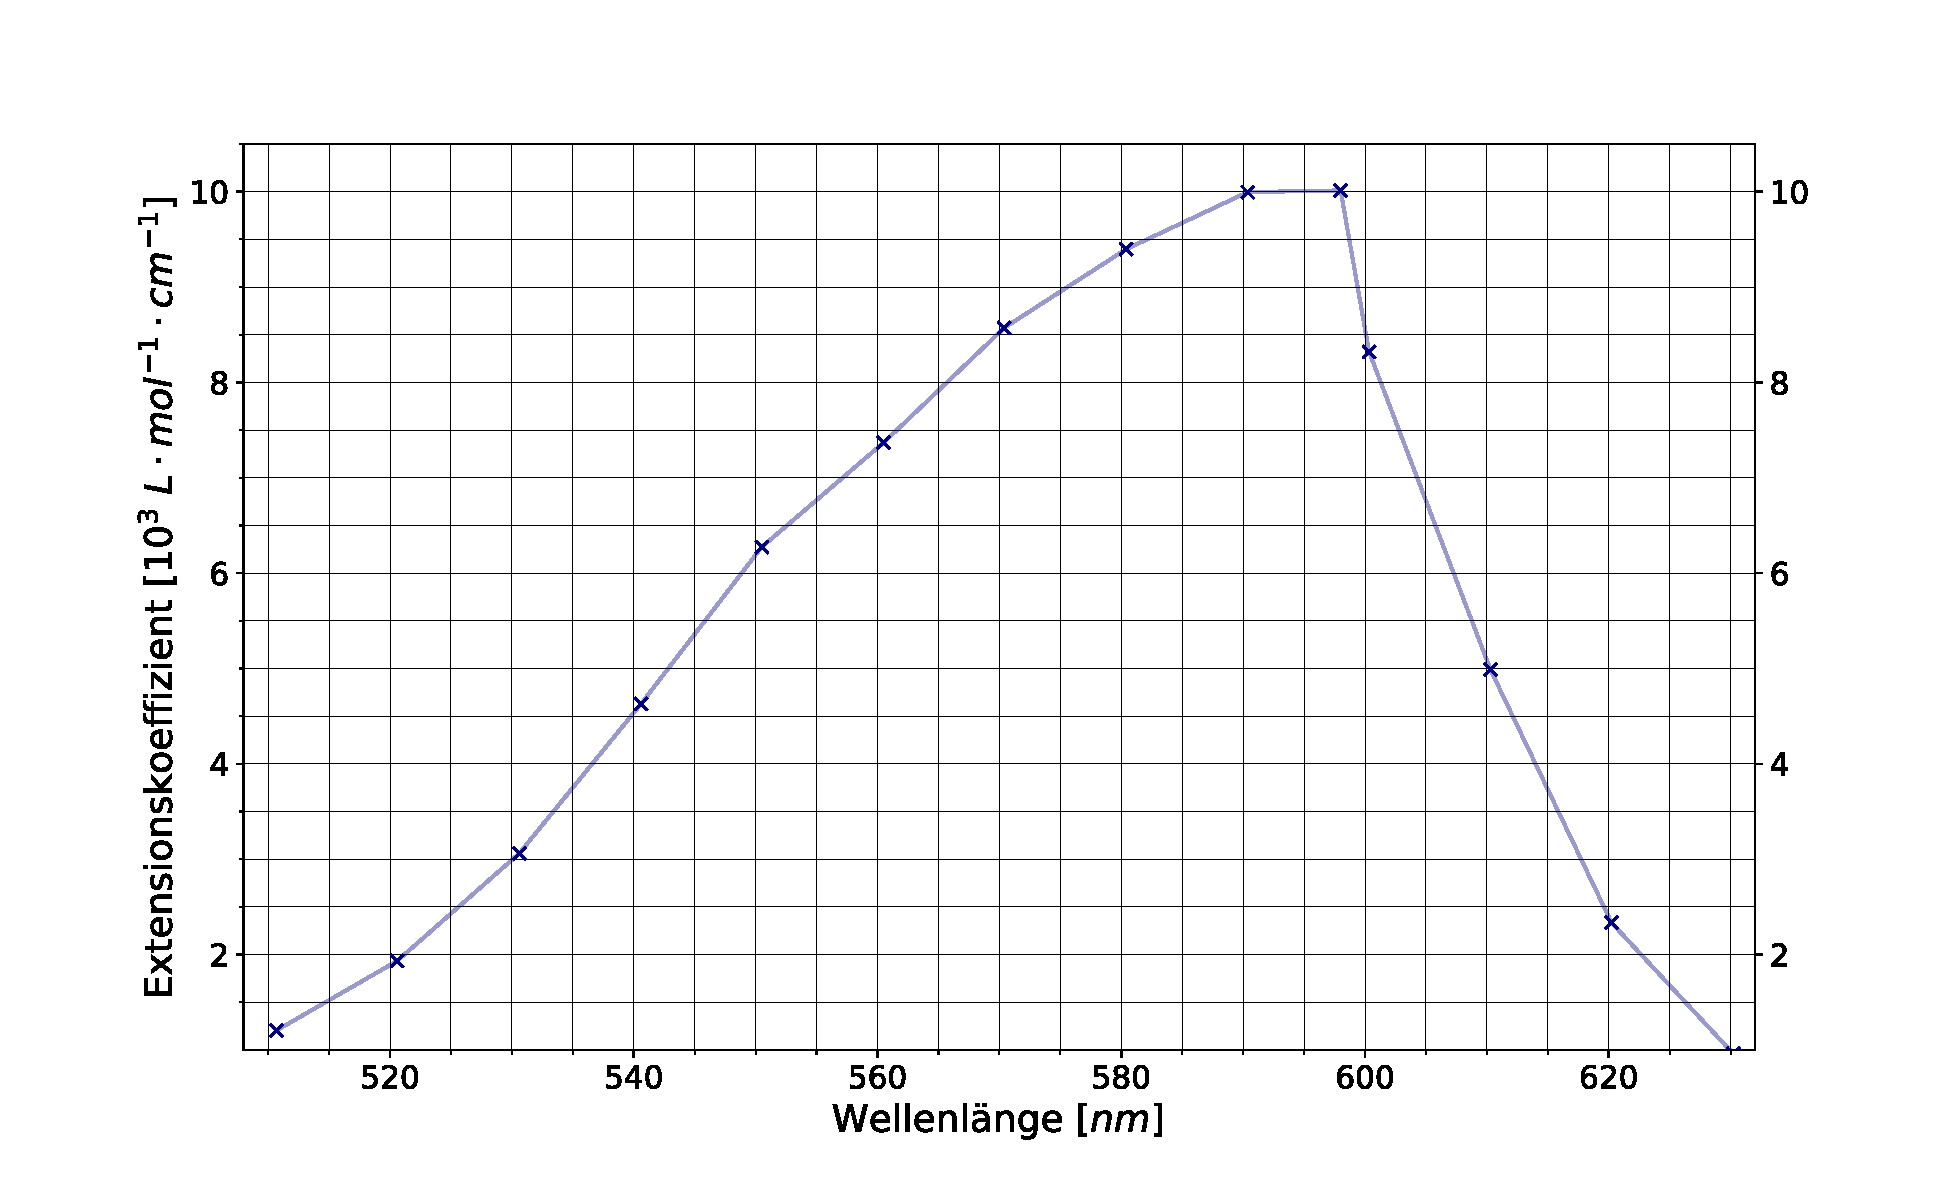
\includegraphics[width=\columnwidth]{Rohdaten/Extkoeff.pdf}	
		\caption{Auftragung der dekadischen Extinktionskoeffizienten über den untersuchten Wellenlängen. Kreuze verdeutlichen die erhaltenen Werte und Linien die zu erwartenden dekadischen Extinktionskoeffizienten für alle weiteren Wellenlängen als Kurve unter der Annahme eines linearen Verhältnisses zwischen den errechneten Werten}
		\label{fig:ExtKoeffs}
	\end{minipage}
\end{figure}
Zwar sind die verschiedene Werte für die untersuchten Wellenlängen diskret, es kann jedoch unter Annahme eines linearen Verhaltens zwischen den Wellenlängen eine genäherte Kurve erhalten werden. Durch diese Kurve können Aussagen über alle weiteren Wellenlängen unter Näherung einer hoch verdünnten Lösung getroffen werden.\\
\\
\textbf{Fehlerbetrachtung}\\
Wie bereits am Anfang dieses Abschnitts erwähnt, wurde der Fehler des durchgeführten Experimentes vor allem durch das Abwiegen des Kristallvioletts gegeben. Die verwendete Wage als \textit{electronic balance} Modell von \textit{KERN \& Sohn GmbH} zeigte beim abwiegen einer Mikrodosis der Substanz eine große Schwankung des Gewichts. Ebenfalls konnte beim Umschütten der Substanz vom Wegepapier in das Versuchsgefäß nicht sichergestellt werden, dass die gesamte Menge überführt wurde. Diese beiden stark fehlerbehafteten Vorgänge für eine sehr kleine Menge an Substanz lässt eine ebenfalls stark fehlerbehaftete Konzentration resultieren. Da in Abbildung \ref{fig:KonzgegenExt} ein linearer Verlauf der Ausgleichsgerade bei geringen Konzentrationen vorliegt, kann vermutet werden, dass die Unsicherheit in der Konzentration keinen Fehler auf die Ergebnisse folgen lässt. Da die Stammlösung bereits vor Beginn des Experiments eine fehlerbehaftete Konzentration besaß stimmen zwar die vorliegenden Konzentrationen nicht, jedoch die erhaltenden Trends der molaren dekadischen Extinktionskoeffizienten aus der Rechnung. 